\chapter{Humanitarian}

\section*{Number of people reached with humanitarian assistance (food aid, cash and voucher transfers) through DFID support.}
% make sure numbers and header don't appear

\thispagestyle{empty}



\section{Results}
From 2015 to March 2020 DFID reached \textbf{
33.7 million
} people with humanitarian assistance (food aid, cash and voucher transfers). %
This is a 1 million person (3\%) increase on the achieved reach from 2015 to March 2019, reported in July 2019. %

From 2015 to 2020 Africa was the largest beneficiary of DFID's humanitarian assistance programmes, with
18.4 million
people reached --- approximately 5 out of every 10 people reached throughout the reporting period. %
The largest number of beneficiaries reached by DFID supported humanitarian programmes in a single African country was in Somalia (3.6 million
people received humanitarian assistance). %

In the Middle East region DFID provided humanitarian assistance to
9
million beneficiaries, the majority of whom were located in Yemen (6.9
million people). %
More people were reached by DFID humanitarian programmes in Yemen, than in any other country. %

A further
4.2
million beneficiaries were from Asia. %
This includes
1.5
million people in Bangladesh and
1.6
million people in Pakistan. %

Finally,
0.5 million
people were assisted in Europe --- in the Ukraine and Turkey --- and
1.4
million people were reached via non-country specific and non-region specific programmes. %

\begin{figure}[htbp]
	\centering
\begin{knitrout}
\definecolor{shadecolor}{rgb}{0.969, 0.969, 0.969}\color{fgcolor}
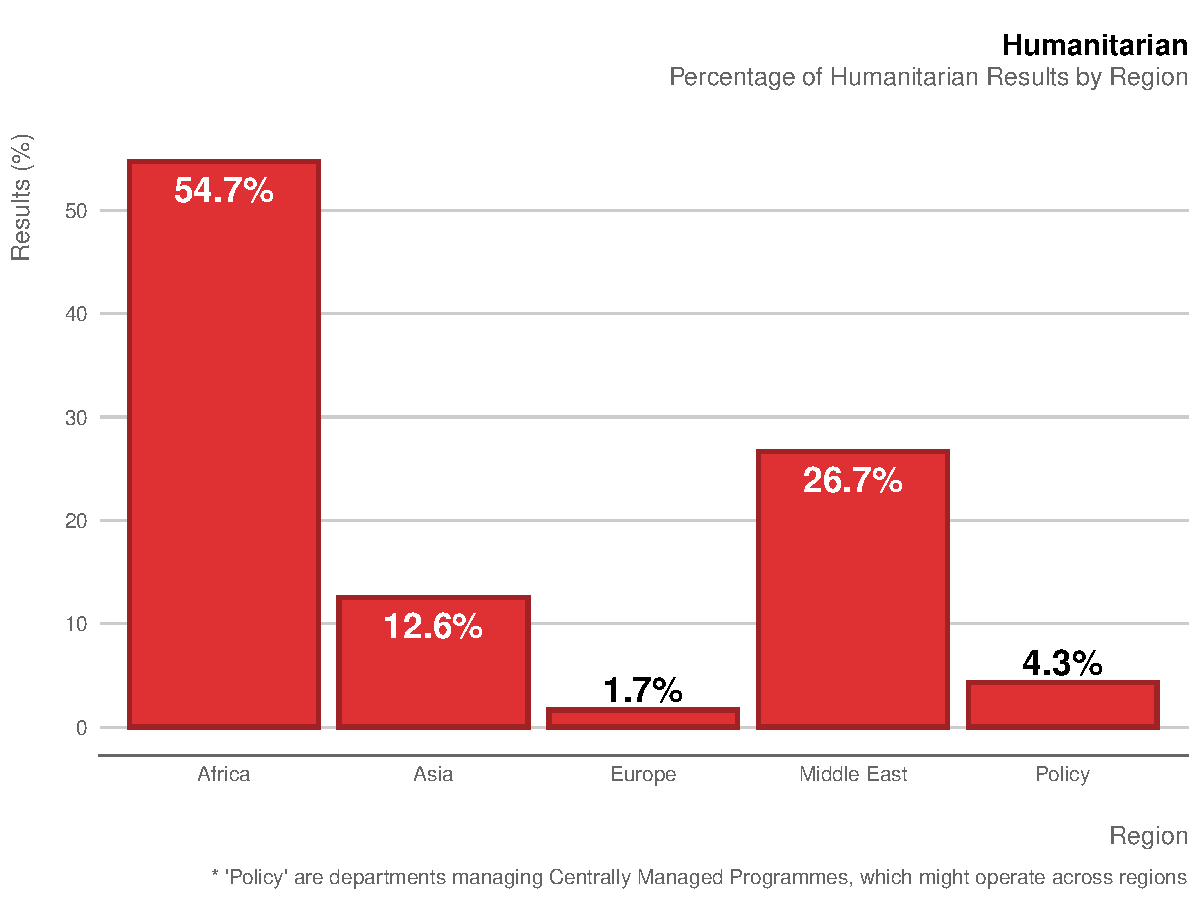
\includegraphics[width=0.8\textwidth]{figs/human_region_plot-1} 

\end{knitrout}
	%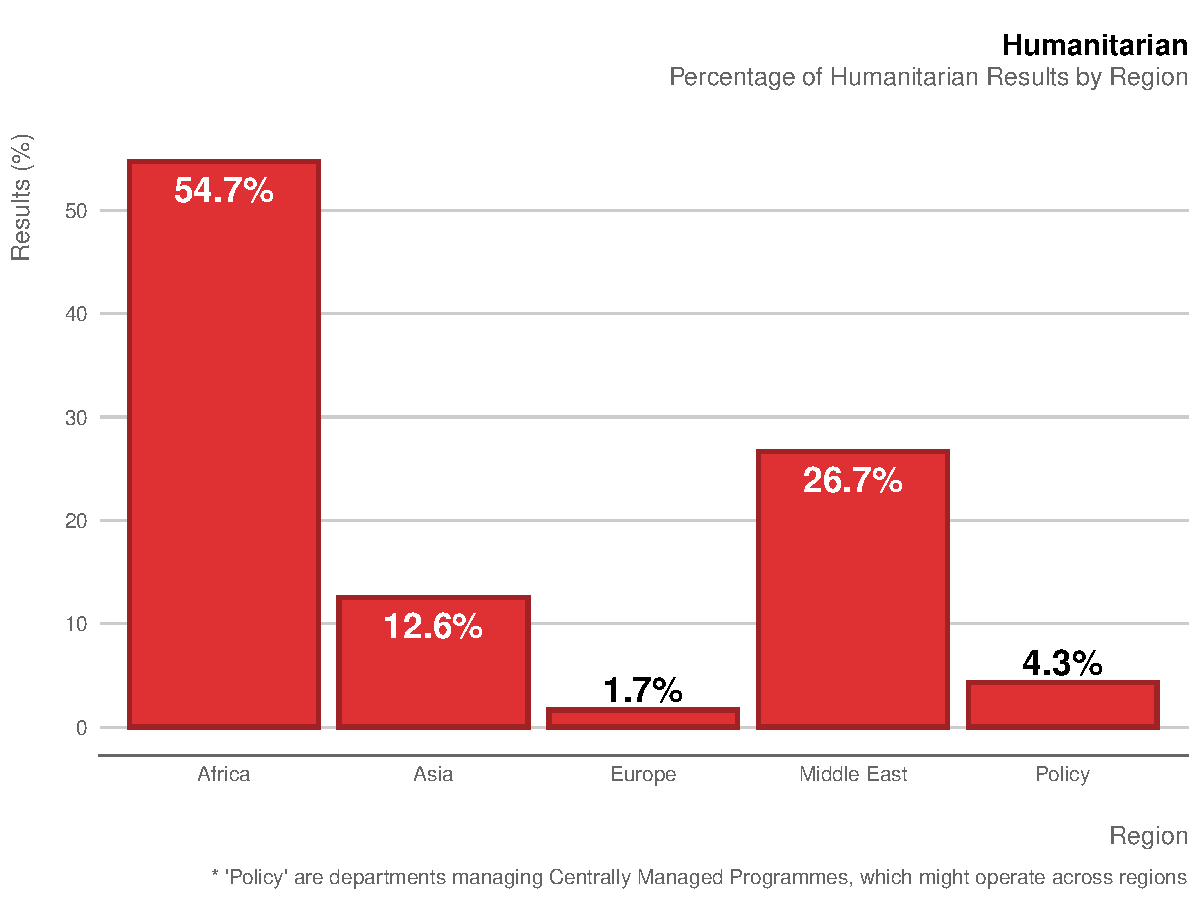
\includegraphics[width=0.8\textwidth]{../figs/human_region_plot} \hfill
	\caption{Percentage of Humanitarian results by region.}
	\label{fig:human_region_plot}
\end{figure}


Over 85\%
(28.7 million beneficiaries
) of the people reached by DFID supported humanitarian assistance live in fragile states (using the OECD States of Fragility definition). %
This includes
18.1
million beneficiaries living in Extremely Fragile states. %
A further
10.6\%
(3.6
million beneficiaries) of DFID supported humanitarian assistance was delivered via non-country specific programmes and so it is not possible to assign a fragility level to these results. %


\begin{figure}[htbp]
	\centering
\begin{knitrout}
\definecolor{shadecolor}{rgb}{0.969, 0.969, 0.969}\color{fgcolor}
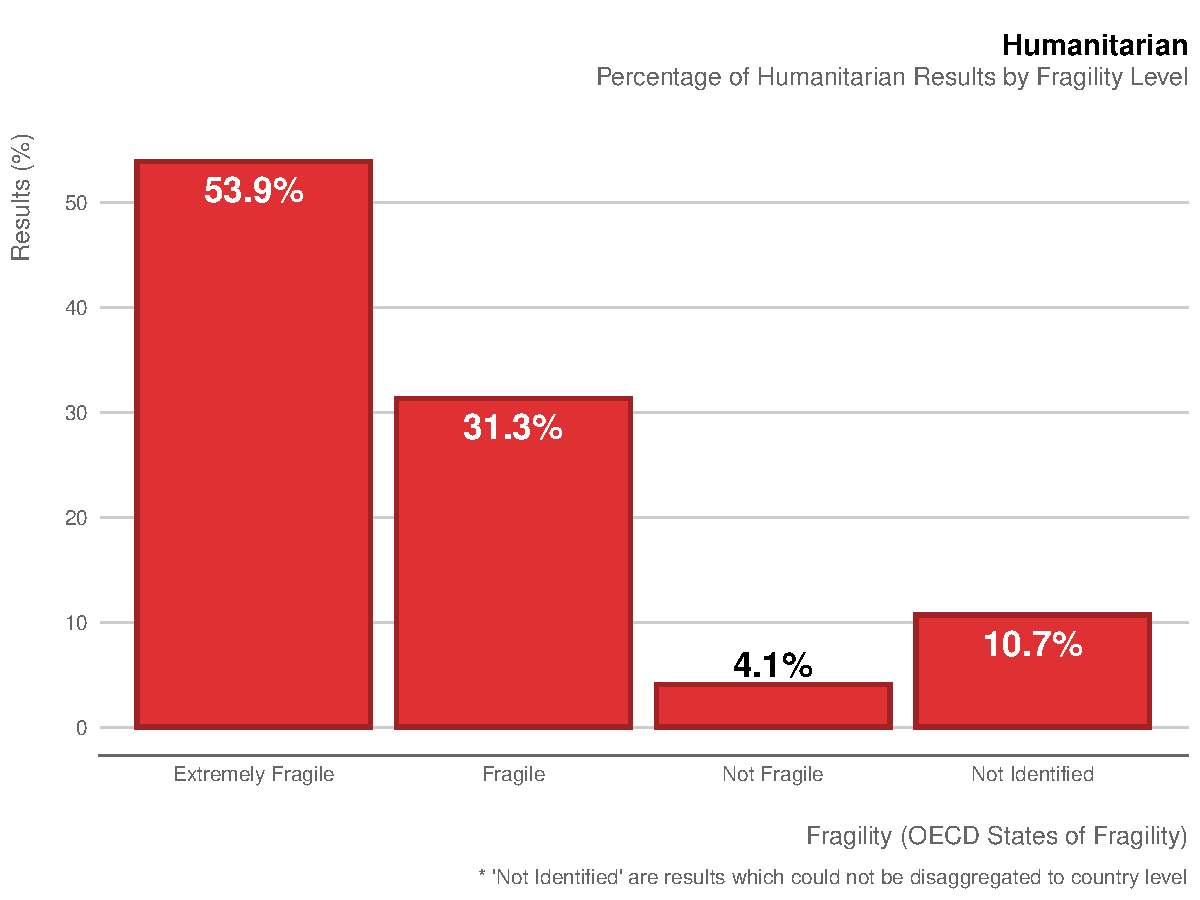
\includegraphics[width=0.8\textwidth]{figs/human_fragility_plot-1} 

\end{knitrout}
	%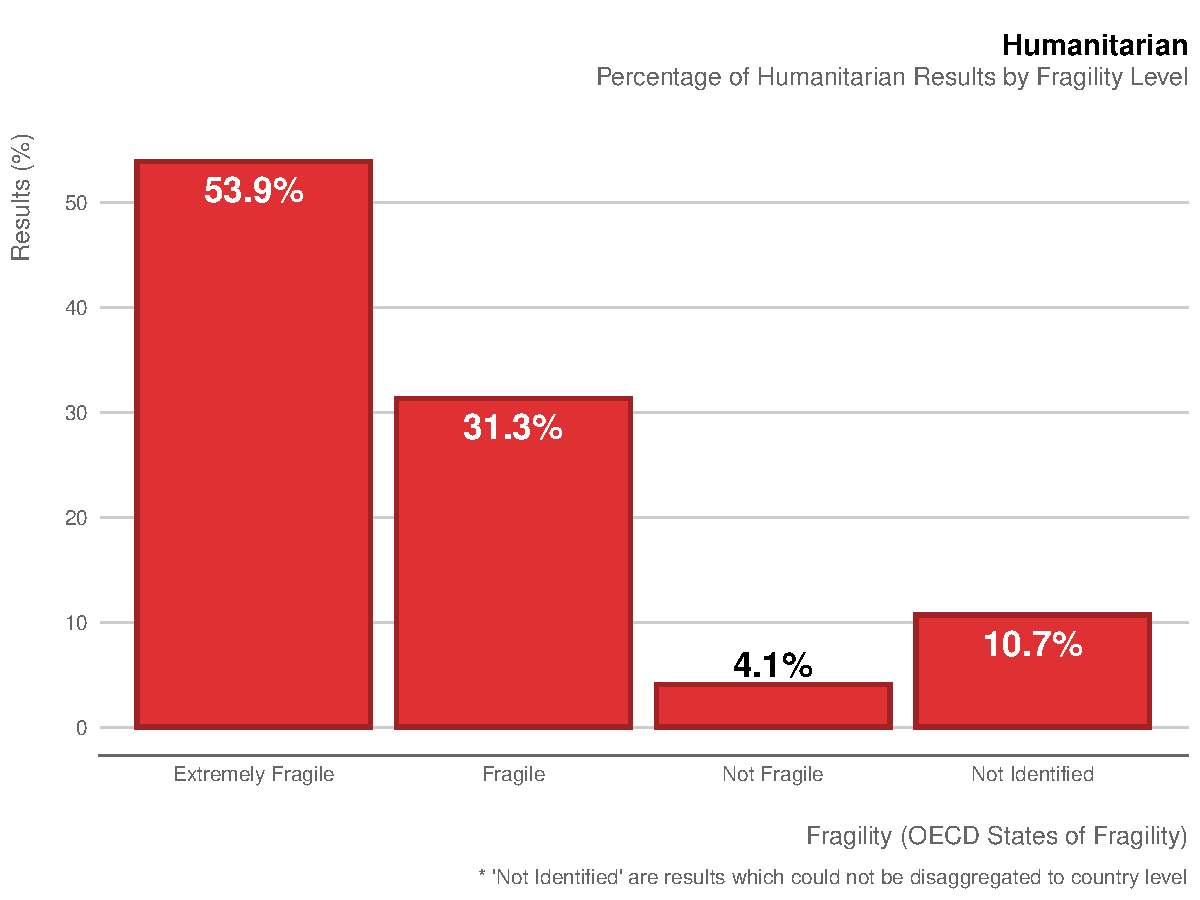
\includegraphics[width=0.8\textwidth]{../figs/human_fragility_plot} \hfill
	\caption{Percentage of Humanitarian results by fragility level.}
	\label{fig:human_fragility_plot}
\end{figure}


Of those reached by DFID humanitarian programmes from 2015 to March 2020, at least
40\% (13.7
million) were women and girls. %

DFID is continuously working with our existing partners towards improving collection of disaggregated data. %
In 2019/20, 76\% of our reported humanitarian results were disaggregated by gender. %
This is a 19 percentage point increase in data disaggregation by gender between the results reported in 2018/19 and 2019/20. %
There are considerable challenges with robust data collection in humanitarian contexts, particularly for people in greatest need. %
These are the generally the most unstable situations in which DFID supported programmes operate, where ongoing conflicts substantially increase the risks faced by those delivering emergency assistance and severely hinder access. %
DFID is collaborating with external partners to develop guidance, support and tools to facilitate data disaggregation but it should be recognised that DFID's commitment to reach those people in greatest need means that data collection and reliable disaggregation in the most difficult humanitarian contexts will continue to be a considerable challenge. %


\section{Context}

Humanitarian aid provides essential material and support assistance to the world's most vulnerable people. %
It is usually short-term help provided in crisis situations to help victims of natural disasters, wars and famines. %
Humanitarian aid saves lives, relieves suffering and maintains human dignity. %
It differs from development aid, which seeks to address the underlying causes which may have led to a crisis or emergency. %

By its nature, humanitarian assistance is reactive to unplanned events, therefore, DFID has no specific targets for the amount of humanitarian assistance to be delivered. %
Instead, DFID focuses on delivering the best possible humanitarian assistance to people in need. %
By working with global and UK partners DFID endeavours to improve the UK's capacity to deliver timely, efficient, effective and equitable humanitarian aid, whenever and wherever it is needed. %
DFID recognises that this assistance should not just be delivered after an event when a crisis has been declared. %
Preventative action and early intervention are more effective --- delivering greater impact for a lower total investment, and preventing unnecessary suffering and loss of life in the early stages of a crisis. %
DFID is working to make responses more predictable and to help countries build resilience, prepare for crises, and manage the risk of crises through tools such as risk insurance. %

The United Nations Office for the Co-ordination of Humanitarian Affairs (OCHA) estimated that over 131.7 million people were in need of humanitarian aid in 2019\footnote{\href{https://www.unocha.org/sites/unocha/files/GHO-2020_v9.1.pdf}{https://www.unocha.org/sites/unocha/files/GHO-2020\_v9.1.pdf}}. %
The persisting drivers of increasing humanitarian need are conflict and protracted violence, while natural disasters, droughts, floods and hurricanes continue to create humanitarian need. %

In the 2019 period, 117.4 million people were targeted globally for humanitarian assistance. %
Fifty-four percent of the \$29.7bn financial requirement was met, leaving unmet requirements, or a funding gap, of \$13.7bn. %

In 2019, the UK provided \pounds 1.5bn in bi-lateral humanitarian aid, 9.9 \% of the total UK official development assistance (ODA) spend. %
This represents an increase of \pounds 208 million compared with 2018 and was partly driven by UK responses to humanitarian crises, for example in Yemen. %
These are provisional figures from Statistics in International Development; the full release in autumn 2020 will confirm final figures and DFID's share of total spend. %
In 2018, humanitarian assistance was the UK's second largest area of spend, after health, on sector specific ODA --- \pounds 1,299 million (8.9 \% of UK ODA). %
DFID was responsible for around 99\% of the total UK ODA spend on humanitarian assistance. %

In addition to crisis or country specific spend the UK continues to be one of the largest contributors of core funding to the UN humanitarian agencies and the Red Cross movement, allowing these partners the flexibility to plan, invest in their capacity for timely and equitable humanitarian responses, and to direct resources to where the need is greatest. %
Recognising the UK's role as donors in delivering the vision of a more effective system in the face of unprecedented humanitarian needs worldwide, UK core funding was redesigned to create incentives for multilateral organisations to perform better. %
From 2018, 30\% of the UK's core funding to humanitarian agencies has been performance-based --- an approach known as ``Payment by Results'' (PbR) --- dependent on the delivery of vital reforms agreed at the World Humanitarian Summit in 2016, including the 'Grand Bargain'. %
In order to trigger full payment, agencies will have to demonstrate they have reformed their working practices in line with commitments to improve the effectiveness and efficiency of the international humanitarian system. %
The targets under PbR are ambitious and incentivise the UN and Red Cross movement to each work more collaboratively. %

In October 2017 the UK set out the new Humanitarian Reform Policy\footnote{\href{https://www.gov.uk/government/publications/uk-governments-humanitarian-reform-policy}{https://www.gov.uk/government/publications/uk-governments-humanitarian-reform-policy}} explaining both innovations and improvements in the UK's humanitarian response, and pushing for a more ambitious reform of the international humanitarian system. %
The UK will:
\begin{itemize}
\item Continue to protect people in crises: upholding humanitarian law and principles, uphold humanitarian law, and support our partners to do the same.
\item Deliver bigger, better, faster responses to rapid onset disasters when national systems are overwhelmed, as demonstrated in the Caribbean.
\item Invest in resilience and preparedness to respond, including using insurance and other risk-based finance to better manage risks from natural hazards.
\item Adopt a new long-term approach to protracted crises, including support to countries hosting long-term refugees to generate livelihoods, trading opportunities and invest in people's future.
\item Challenge the international humanitarian system to hold itself to account for delivering better for people affected by crises, and ensuring the most vulnerable people in the world are appropriately protected from environmental and social hazards.
\item Ensure that response is delivered through organisations and mechanisms which offer best value for money, such as encouraging the use of multi-purpose cash transfers (where appropriate) which are faster, safer and more cost-effective than relief-in kind whilst providing additional support to local economies.
\end{itemize}

Single departmental plan results are attributed from DFID bi-lateral programmes and do not include the UK contribution to results attributed to UN or Red Cross agency central programmes where DFID is not a specific project partner. %


\newpage
